\chapter{Mobilná aplikácia}
\label{chap:mobilna-aplikacia}

Ústredný bod systému Apk Analyzer tvorí mobilná aplikácia, ktorá analyzuje nainštalované aplikačné balíčky. Táto aplikácia poskytuje užívateľovi podrobné informácie o jeho aplikáciách a umožňuje mu kontrolu originality aplikácie. Vyvinutá aplikácia je od októbra 2017 dostupná v oficiálnom obchode Google Play Store~\cite{gp}. Táto kapitola obsahuje popis vyvinutej aplikácie, spolu s technikami získavania informácií o aplikačných balíčkoch v operačnom systéme Android.

\section{Ciele a požiadavky kladené na aplikáciu}
Pre platformu Android je dostupných viacero aplikácií schopných analyzovať softvérový obsah zariadenia. Hlavnou motiváciou je vytvorenie novej mobilnej aplikácie, ktorá má predpoklady presadiť sa medzi ostatnými podobnými riešeniami. Cieľom je implementovať aplikáciu, ktorá sa v Google Play Store dostane medzi najsťahovanejšie a najlepšie hodnotené aplikácie analyzujúce aplikačné balíčky. Za týmto účelom je potrebné nie len vylepšiť nedostatky existujúcich aplikácií, ale aj poskytnúť nové funkcie, atraktívny dizajn a prehľadné užívateľské rozhranie. 

\subsection{Existujúce riešenia a ich nedostatky}
Oficiálny obchod \zv{Google Play Store} obsahuje viaceré aplikácie schopné analyzovať nainštalované aplikačné balíčky. V obchode sa nachádzajú aplikácie s názvom \zv{Apk Analyzer}, \zv{App Info} alebo \zv{App Detective}. Najpopulárnejšie z týchto aplikácií dosahovali v januári 2018 viac ako $50\,000$ celkových inštalácií~\cite{kfOvdBmwje56iW6j}. Pred začiatkom vývoja novej aplikácie bol vykonaný detailný rozbor existujúcich riešení, s dôrazom na identifikáciu nedostatkov, ktoré by mohli byť v novo vyvinutej aplikácií odstránené.
\subsubsection{\textbf{Používateľské rozhranie}}
Väčšina aplikácií zameriavajúcich sa na analýzu softvérového obsahu zariadenia nedodržiava základné princípy dizajnu používateľského rozhrania. Pri niektorých aplikáciách je to spôsobené ich starším časom vydania a prispôsobením na staršie verzie systému. No aj veľká časť pravidelne aktualizovaných nových aplikácií sa nedrží doporučených dizajnových princípov, čo má za následok zhoršenie ovládateľnosti a užívateľského dojmu.

\subsubsection{\textbf{Limitované informácie}}
Veľká časť aplikácií, ktorých názov napovedá, že zobrazujú dáta o aplikačných balíčkoch sa zameriava na veľmi malú časť dostupných informácií. Ako príklad môže slúžiť aplikácia \zv{APK ANALYZER} od vydavateľa \zv{z-project}, ktorá zobrazuje len súbor \zv{AndroidManifest.xml}~\cite{kfOvdBmwje56iW6i}. Aplikácia \zv{App Info} zobrazuje informácie výhradne o vyžadovaných bezpečnostných povoleniach~\cite{kfOvdBmwje56iW6i}.

\subsection{Funkčné požiadavky}
Cieľom novo vyvinutej mobilnej aplikácie je vylepšiť identifikované nedostatky a implementovať aplikáciu v súlade so štandardami systému Android. Funkčné požiadavky kladené na mobilnú aplikáciu vychádzajú z jej funkcie v celom navrhnutom systéme Apk Analyzer, kde mobilná aplikácia slúži ako zdroj aplikačných metadát a poskytuje užívateľské rozhranie.


Na základe analýzy podobných aplikácií boli na novú aplikáciu kladené nasledujúce požiadavky, ktoré sa úspešne podarilo zrealizovať.

\subsubsection{\textbf{Získanie podrobných dát o aplikáciách}}
Cieľom aplikácie je získať čo najpodrobnejšie dáta z rôznych častí aplikácie. Získané informácie obsahujú metadáta zo súboru AndroidManifest.xml, údaje o zdrojových súboroch, aplikačných komponentoch, povoleniach, a aj dáta o zdrojovom kóde aplikácie. 

\subsubsection{\textbf{Analýza nenainštalovaných aplikácií}}
Žiadna z existujúcich aplikácií (podľa vedomia autora) v čase návrhu novej aplikácie neposkytovala analýzu aplikácií, ktoré nie sú nainštalované, ale sú prítomné v pamäti zariadenia ako inštalačné APK balíčky. Cieľom je implementovať túto funkcionalitu, ktorá poskytuje konkurenčnú výhodu oproti ostatným podobným aplikáciám.

\subsubsection{\textbf{Štatistiky o aplikáciách v zariadení}}
Na základe dát získaných analýzou, je možné prezentovať užívateľovi štatistické informácie o skupine aplikácií na jeho zariadení.

\subsubsection{\textbf{Zrozumiteľná interpretácia dát}}
Dáta získané pomocou analýzy je potrebné prehľadne zobraziť užívateľovi.  Získané dáta obsahujú množstvo rôznych atribútov APK súboru. Cieľom je prezentovať tieto dáta tak, aby boli zrozumiteľné aj užívateľom, ktorí nie sú v danej problematike expertmi. Každý atribút musí byť preto sprevádzaný krátkym textovým popisom, ktorý je dostupný užívateľovi.

\subsubsection{\textbf{Používateľské rozhranie}}
Aplikácia musí obsahovať prehľadné rozhranie, ktoré je v súlade so štandardami systému Android.

\subsubsection{\textbf{Komunikácia so serverovou časťou systému}}
Mobilná aplikácia komunikuje so serverom, ktorý sprostredkováva funkcionalitu detekcie prebalených aplikácií. Mobilná aplikácia odosiela serveru metadáta o aplikáciách.

\subsection{Nefunkčné požiadavky}
Návrh aplikácie ovplyvňujú dve základné nefunkčné požiadavky.

\subsubsection{\textbf{Aplikácia nevyžaduje \zv{root} zariadenia}}
V prípade rootu zariadenia má užívateľ právo použiť systémové prostriedky, ktoré sú obyčajnému užívateľovi zakázané. Tieto práva môžu byť využité napríklad na priamy prístup do inštalačných adresárov. Limitácia aplikácie na rootnuté zariadenia by výrazne znížila skupinu potenciálnych užívateľov. Preto musí aplikácia pracovať s oprávneniami štandardného užívateľa.

\subsubsection{\textbf{Výkonnosť}}
Analýza aplikácie musí zohľadňovať aspekt časovej náročnosti. Z pohľadu užívateľa je dôležité rýchle zobrazenie informácií o aplikácii. 


\section{Získavanie dát}
Základná funkcionalita aplikácie spočíva v získavaní metadát o aplikáciách. Systém Android poskytuje viacero rozhraní, prostredníctvom ktorých je možné získavať dáta o aplikačných balíčkoch.

\subsection{Package Manager}
Trieda \zv{PackageManager} poskytuje API pre získavanie rôznych dát o nainštalovaných aplikáciách. Aplikácia \zv{Apk Analyzer} využíva metódu \zv{getInstalledPackages()} na získanie zoznamu nainštalovaných aplikácií. 

Pomocou triedy \zv{PackageManager} je získaná veľká časť informácií, ktoré obsahuje metasúbor \zv{AndroidManifest.xml}. Táto trieda poskytuje metódu \zv{getPackageInfo()}, pomocou ktorej je možné získať informácie o nainštalovanom aplikačnom balíčku. Na získanie informácií o nenainštalovaných APK súboroch je možné použiť metódu \zv{getPackageArchiveInfo()}, ktorá na rozdiel od predchádzajúcej metódy analyzuje aplikačný archív, ktorý nemusí byť nainštalovaný.
\\\\
\noindent Pomocou metód \zv{getPackageArchiveInfo()} a \zv{getPackageInfo()} sú z aplikačného balíčka získané nasledujúce údaje:
\begin{itemize}
	\item Základné metadáta aplikácie a informácie dostupné v súbore \zv{AndroidManifest.xml}
	\item Informácie o digitálnom podpise
	\item Komponenty aplikácie
	\item Definované a vyžadované bezpečnostné oprávnenia
	\item Hardvérové vlastnosti zariadenia vyžadované aplikáciou.
\end{itemize}

\subsection{Rekonštrukcia AndroidManifest.xml}
Systém Android neposkytuje aplikačné programové rozhranie na prístup k súboru \zv{AndroidManifest.xml}. Všetky dôležité informácie z tohto súboru sú dostupné pomocou API triedy \zv{PackageManager}. Za účelom získania pôvodného manifest súboru používa aplikácia \zv{Apk Analyzer} riešenie založené na prístupe k zdrojovým súborom. Trieda \zv{PackageManager} poskytuje možnosť prístupu k niektorým zdrojovým súborom aplikácií. \zv{AndroidManifest.xml} je možné nájsť medzi 
zv{asset} súbormi. Pomocou tohto prístupu však nie je možné súbor celý načítať, ale len vytvoriť tzv. pull parser, ktorý služi na spracovanie xml súboru.\\ 
\begin{lstlisting} [language=java, basicstyle=\small\color{black},frame=single,framesep=10pt, caption= {Prístup k súboru AndroidManifest.xml v nainštalovanej aplikácii} \label{code:manifestParse}]
Resources apkResources = packageManager
                         .getResourcesForApplication(packageName);
XmlResourceParser parser = apkResources.getAssets()
                         .openXmlResourceParser("AndroidManifest.xml");
\end{lstlisting}
\mbox{}\\
\noindent Algoritmus následne pomocou tohto objektu spracováva jednotlivé xml elementy a vytvára z nich textovú reprezentáciu tohto súboru.


Takto vytvorený xml súbor však nie je čitateľný. Hodnoty veľkej časti atribútov sa odkazujú na zdrojové súbory, ktoré sú skompilované v rámci súboru \zv{resources.arsc}. Príkladom je xml element \zv{application} v ukážke \ref{xml:manifest-before}.  Téma na ktorú sa tento element odkazuje je aplikácií dostupná pod identifikátorom $78954341$, a názov je dostupný ako textový zdroj číslo $4562348$.
\mbox{}\\
\begin{lstlisting} [language=xml,frame=single,framesep=10pt, caption= {Ukážka AndroidManifest.xml získaného pomocou parsera} \label{xml:manifest-before}]
<application theme="@78954341" label="@4562348" >
\end{lstlisting}
\mbox{}\\
Za účelom eliminovania tohto správania využíva \zv{Apk Analyzer} prístup k zdrojovým súborom analyzovaných aplikácií. V týchto súboroch vyhľadá text korešpondujúci s daným identifikátorom a dosadí ho do vytvorenej textovej reprezentácie súboru \zv{AndroidManifest.xml}. Výsledok tejto operácie je zobrazený na ukážke \ref{xml:manifest-after}.
\mbox{}\\
\begin{lstlisting} [language=xml,frame=single,framesep=10pt, caption= {Ukážka AndroidManifest.xml po substitúcií identifikátorov zdrojových textov} \label{xml:manifest-after}]
<application theme="Theme.YouTube.Light" label="Youtube"/>
\end{lstlisting}

\subsection{Súbory v APK balíčku}
Na získanie zoznamu všetkých súborov v aplikácii spolu s ich identifikátormi v podobe hashu je využitý súbor \cesta{MANIFEST.MF}, ktorý je vytvorený v priebehu tvorby APK balíčka.  Prístup k tomuto súboru je možný prostredníctvom štandardného Java API a triedy \zv{JarFile}.

\subsection{Zdrojový kód}
Dáta \zv{DEX} súboru, ktorý obsahuje zdrojový kód, získava aplikácia pomocou triedy \zv{dalvik.system.DexFile}. Táto trieda obsahuje operácie, pomocou ktorých je možné získať zoznam všetkých aplikačných tried, ktoré má daná aplikácia k dispozícií. Tento zoznam obsahuje triedy samotnej aplikácie, spolu so všetkými použitými knižnicami. 

\section{Aplikácia}
Mobilná aplikácia bola implementovaná v jazyku Java. Je dostupná v obchode \zv{Google Play} pod názvom \zv{Apk Analyzer}, a je unikátne identifikovaná pomocou mena balíku \zv{sk.styk.martin.apkanalyzer}~\cite{gp}. Aplikácia je dostupná pre všetky zariadenia s verziou systému novšou ako Android 4.0.3 (API level 15) a  je prispôsobená na použitie na mobilných telefónoch a tabletoch. Nasledujúce sekcie opisujú hlavnú funkcionalitu aplikácie.



\subsection{Zoznam nainštalovaných aplikácií}
\begin{figure}[H]
\begin{minipage}[t]{0.48\textwidth}
Základná obrazovka obsahuje zoznam všetkých nainštalovaných aplikačných balíčkov. Tento zoznam sa užívateľovi zobrazí po spustení aplikácie. V zozname aplikácií je možné vyhľadávať podľa lokalizovaného názvu aplikácie alebo mena balíčku. Taktiež je možné filtrovať aplikácie na základe ich pôvodu. Táto funkcia poskytuje užívateľom možnosť ľahko rozlíšiť medzi aplikáciami získanými z oficiálneho obchodu a z alternatívnych zdrojov. Kliknutím na položku zoznamu sa zobrazia detailné informácie o vybranej aplikácií. V prípade analýzy nenainštalovaného aplikačného balíčku, vyberie užívateľ APK súbor z pamäte zariadenia pomocou tlačidla umiestneného v pravom dolnom rohu obrazovky.
\end{minipage}%
\hfill
\centering
\begin{minipage}[t][][b]{0.45\textwidth}
\centering
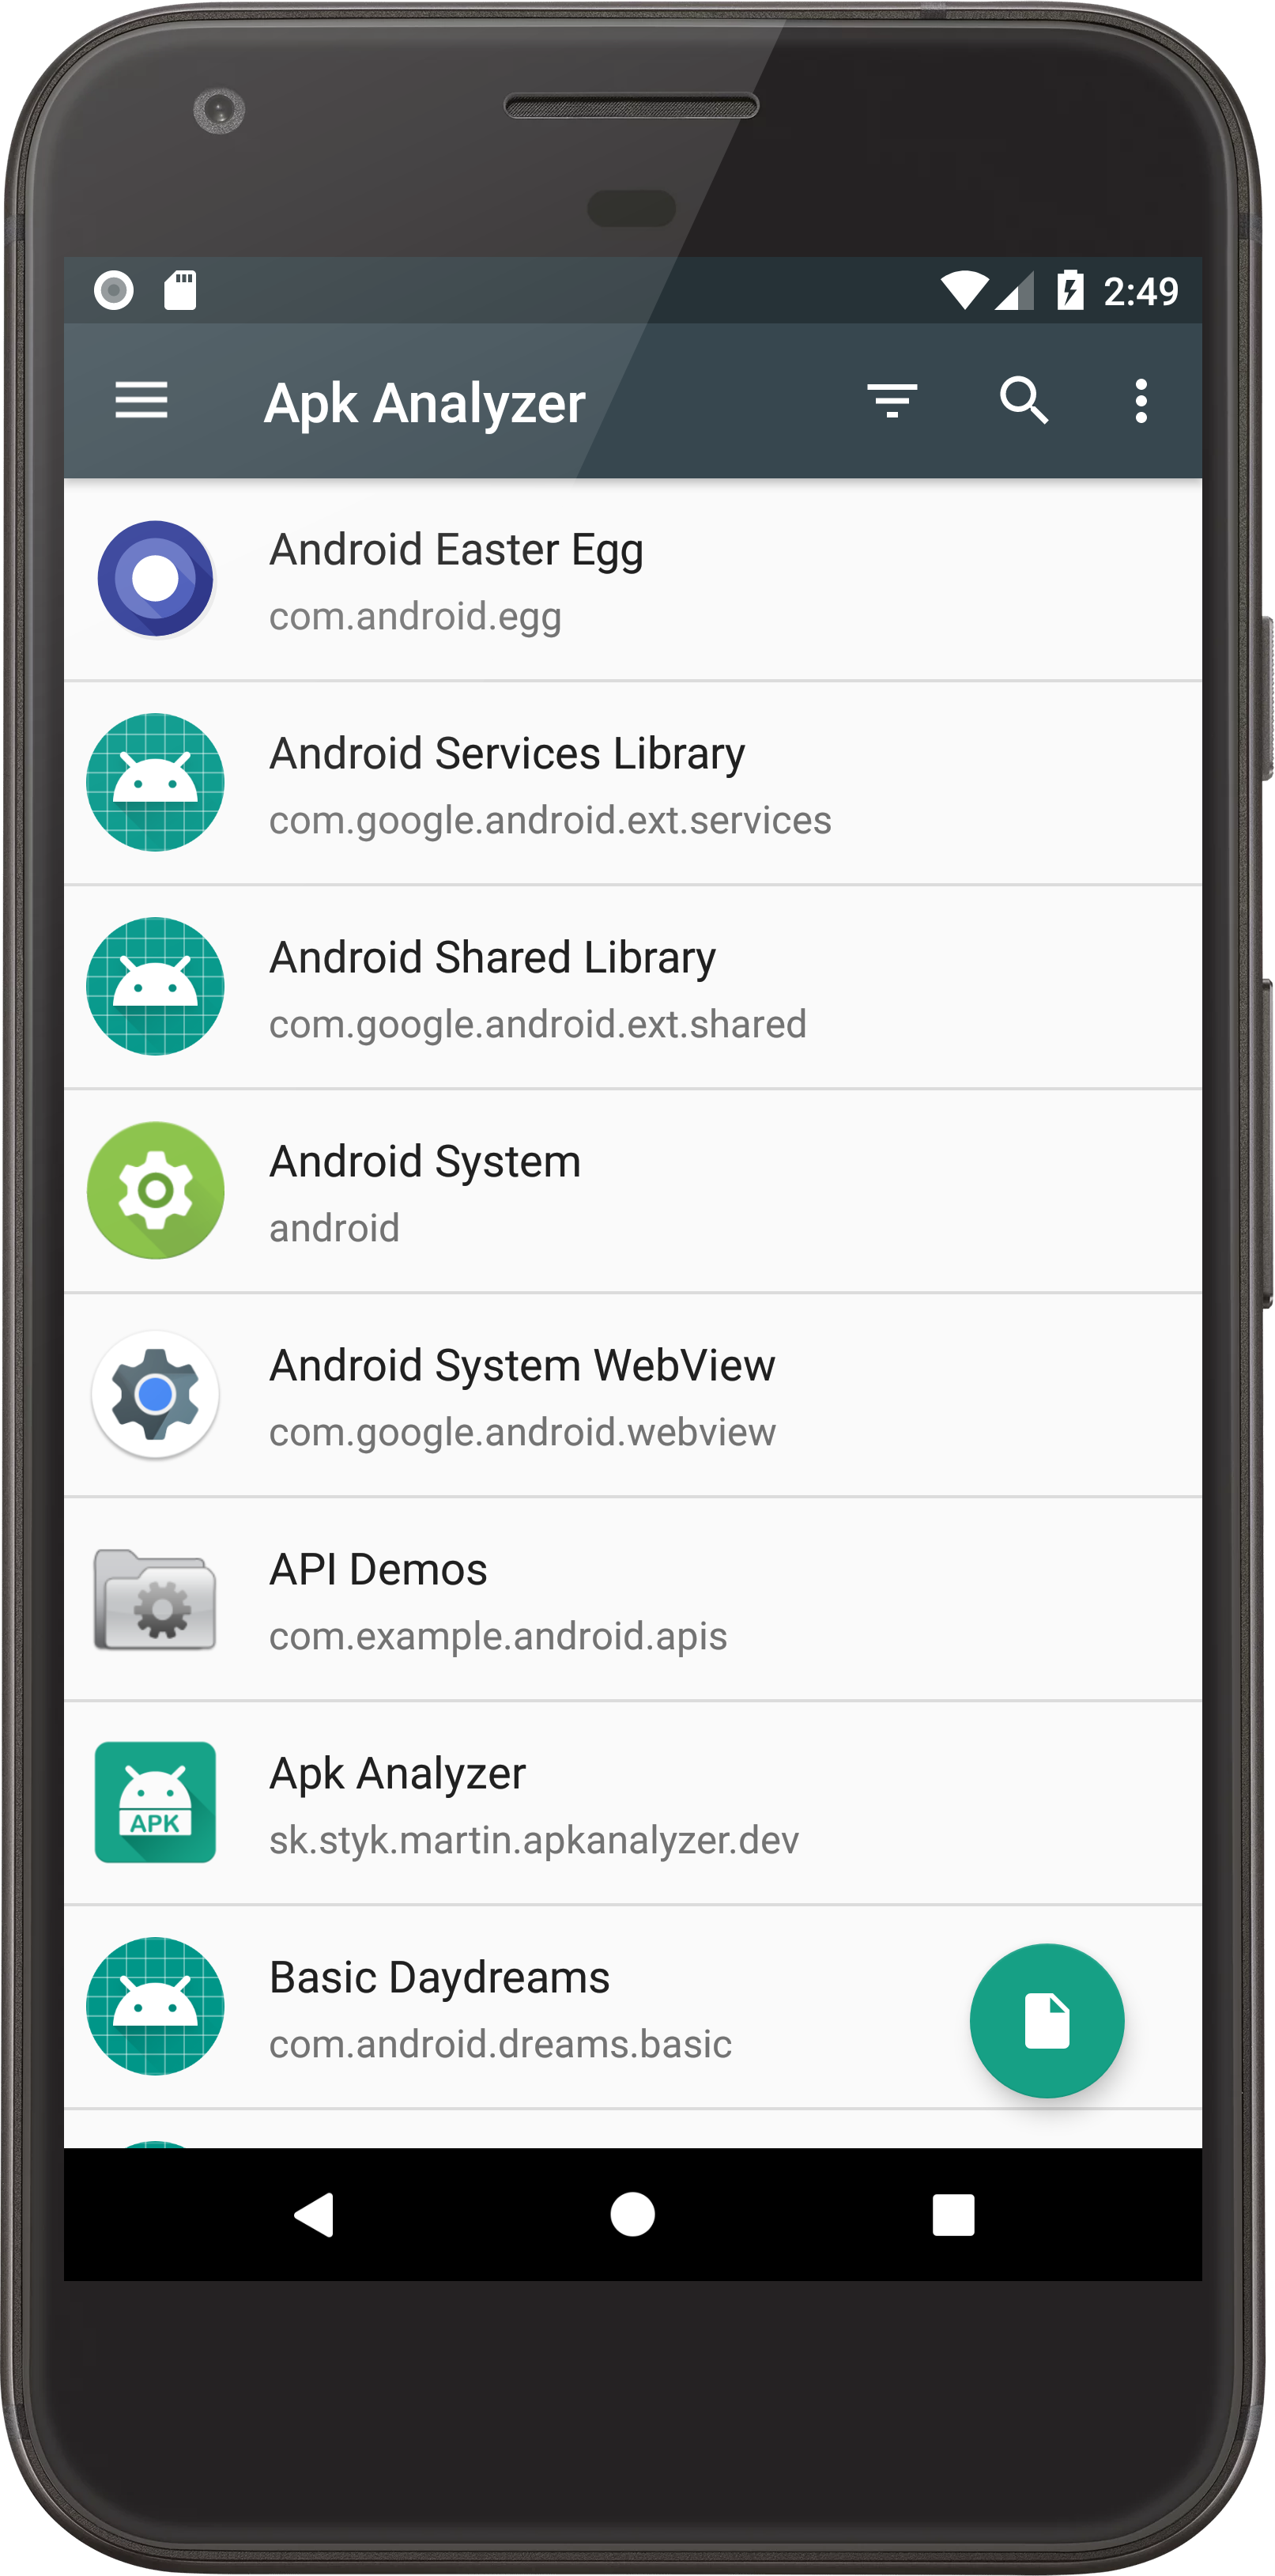
\includegraphics[width=5.2cm]{images/app/list_device.png}
\centering
\caption{Zoznam nainštalovaných aplikácií}
\label{fig:app-list}
\end{minipage}%
\end{figure}

\subsection{Analýza aplikácie}
Táto obrazovka zobrazuje dáta získané analýzou aplikačného balíčku. Z dôvodu veľkého počtu atribútov získaných analýzou, sú tieto dáta zobrazené vo viacerých záložkách, medzi ktorými môže užívateľ prepínať. 
\\
\noindent Atribúty analyzovaných aplikácií sú rozdelené tematicky do nasledujúcich skupín:
\begin{itemize}
	\item \bod{Všeobecné informácie} -- základne dáta o aplikácií, napr. názov, verzia, zdroj alebo kompatibilné vezie systému Android
	\item \bod{Informácie o podpise APK balíčka} -- dáta získané zo súborov v adresári META-INF. Atribúty v tejto kategórií obsahujú dobu platnosti certifikátu, názov vydavateľa, alebo algoritmus podpisu APK balíčka
	\item \bod{Informácie o zdrojových súboroch} -- zastúpenie rôznych formátov a veľkostí zdrojových súborov. Tieto informácie je možné získať iba pokiaľ aplikácia nevyužíva obfuskáciu názvov súborov a adresárov
	\item \bod{Informácie komponentoch aplikácie} -- dáta o aktivitách, službách, poskytovateľoch obsahu a prijímačoch definovaných aplikáciou. V prípade verejne dostupných aktivít, poskytuje aplikácia možnosť ich priameho spustenia. Užívateľ tak môže priamo spustiť rôzne časti iných aplikácií.
	\item \bod{Používané hardvérové vlastnosti} -- zoznam vlastností definovaných v súbore AndroidManifest.xml v rámci elementu feature
	\item \bod{Vyžadované bezpečnostné povolenia} -- zoznam povolení definovaných v súbore AndroidManifest.xml v rámci elementu uses-permission
	\item \bod{Definované bezpečnostné povolenia} -- zoznam povolení definovaných v súbore AndroidManifest.xml v rámci elementu defines-permission
	\item \bod{DEX súbor} -- zoznam všetkých Java a Kotlin tried, ktoré sú zabalené v DEX súbore danej aplikácie
\end{itemize}
Kompletný zoznam atribútov získaných pomocou analýzy obsahuje príloha \ref{ziskaneDataPriloha}. 

Po kliknutí na položku atribútu analyzovanej aplikácie sa zobrazí popis daného atribútu. Na základe tohto popisu môže dáta zmysluplne interpretovať aj užívateľ, ktorý nie je odborníkom v oblasti aplikácií pre systém Android.

Táto obrazovka poskytuje užívateľovi prístup k ďalším informáciám a operáciám s analyzovanou aplikáciou. Medzi najdôležitejšie patrí možnosť zobrazenia súboru \zv{AndroidManifest.xml} danej aplikácie. Manifest je možné uložiť do externej pamäte zariadenia. Prístup k súboru \zv{AndroidManifest.xml} je možny len pri analýze nainštalovanej aplikácie.
\begin{figure}[H]
\begin{minipage}[t]{0.48\textwidth}
Užívateľ môže exportovať APK súbor nainštalovanej aplikácie. Systém Android ukladá inštalačné súbory všetkých aplikácií do priečinka, ktorý nie je bežným užívateľom prístupný. Pomocou funkcie exportu APK súboru dokáže naša aplikácia skopírovať tento súbor do užívateľovi prístupnej časti úložného priestoru. Aplikácia taktiež poskytuje možnosť zdieľania APK súborov. 
\zv{Apk Analyzer} sa nezameriava na získavanie dát o konkrétnej inštalácii aplikácie. Tieto dáta poskytuje systémová aplikácia, ktorá je súčasťou štandardných Android nastavení. Naša aplikácia poskytuje možnosť priameho prechodu na túto systémovú aplikáciu.  Taktiež poskytuje možnosť zobrazenia záznamu o aplikácií na obchode \zv{Google Play}.
\end{minipage}%
\hfill
\centering
\begin{minipage}[t][][b]{0.45\textwidth}
\centering
    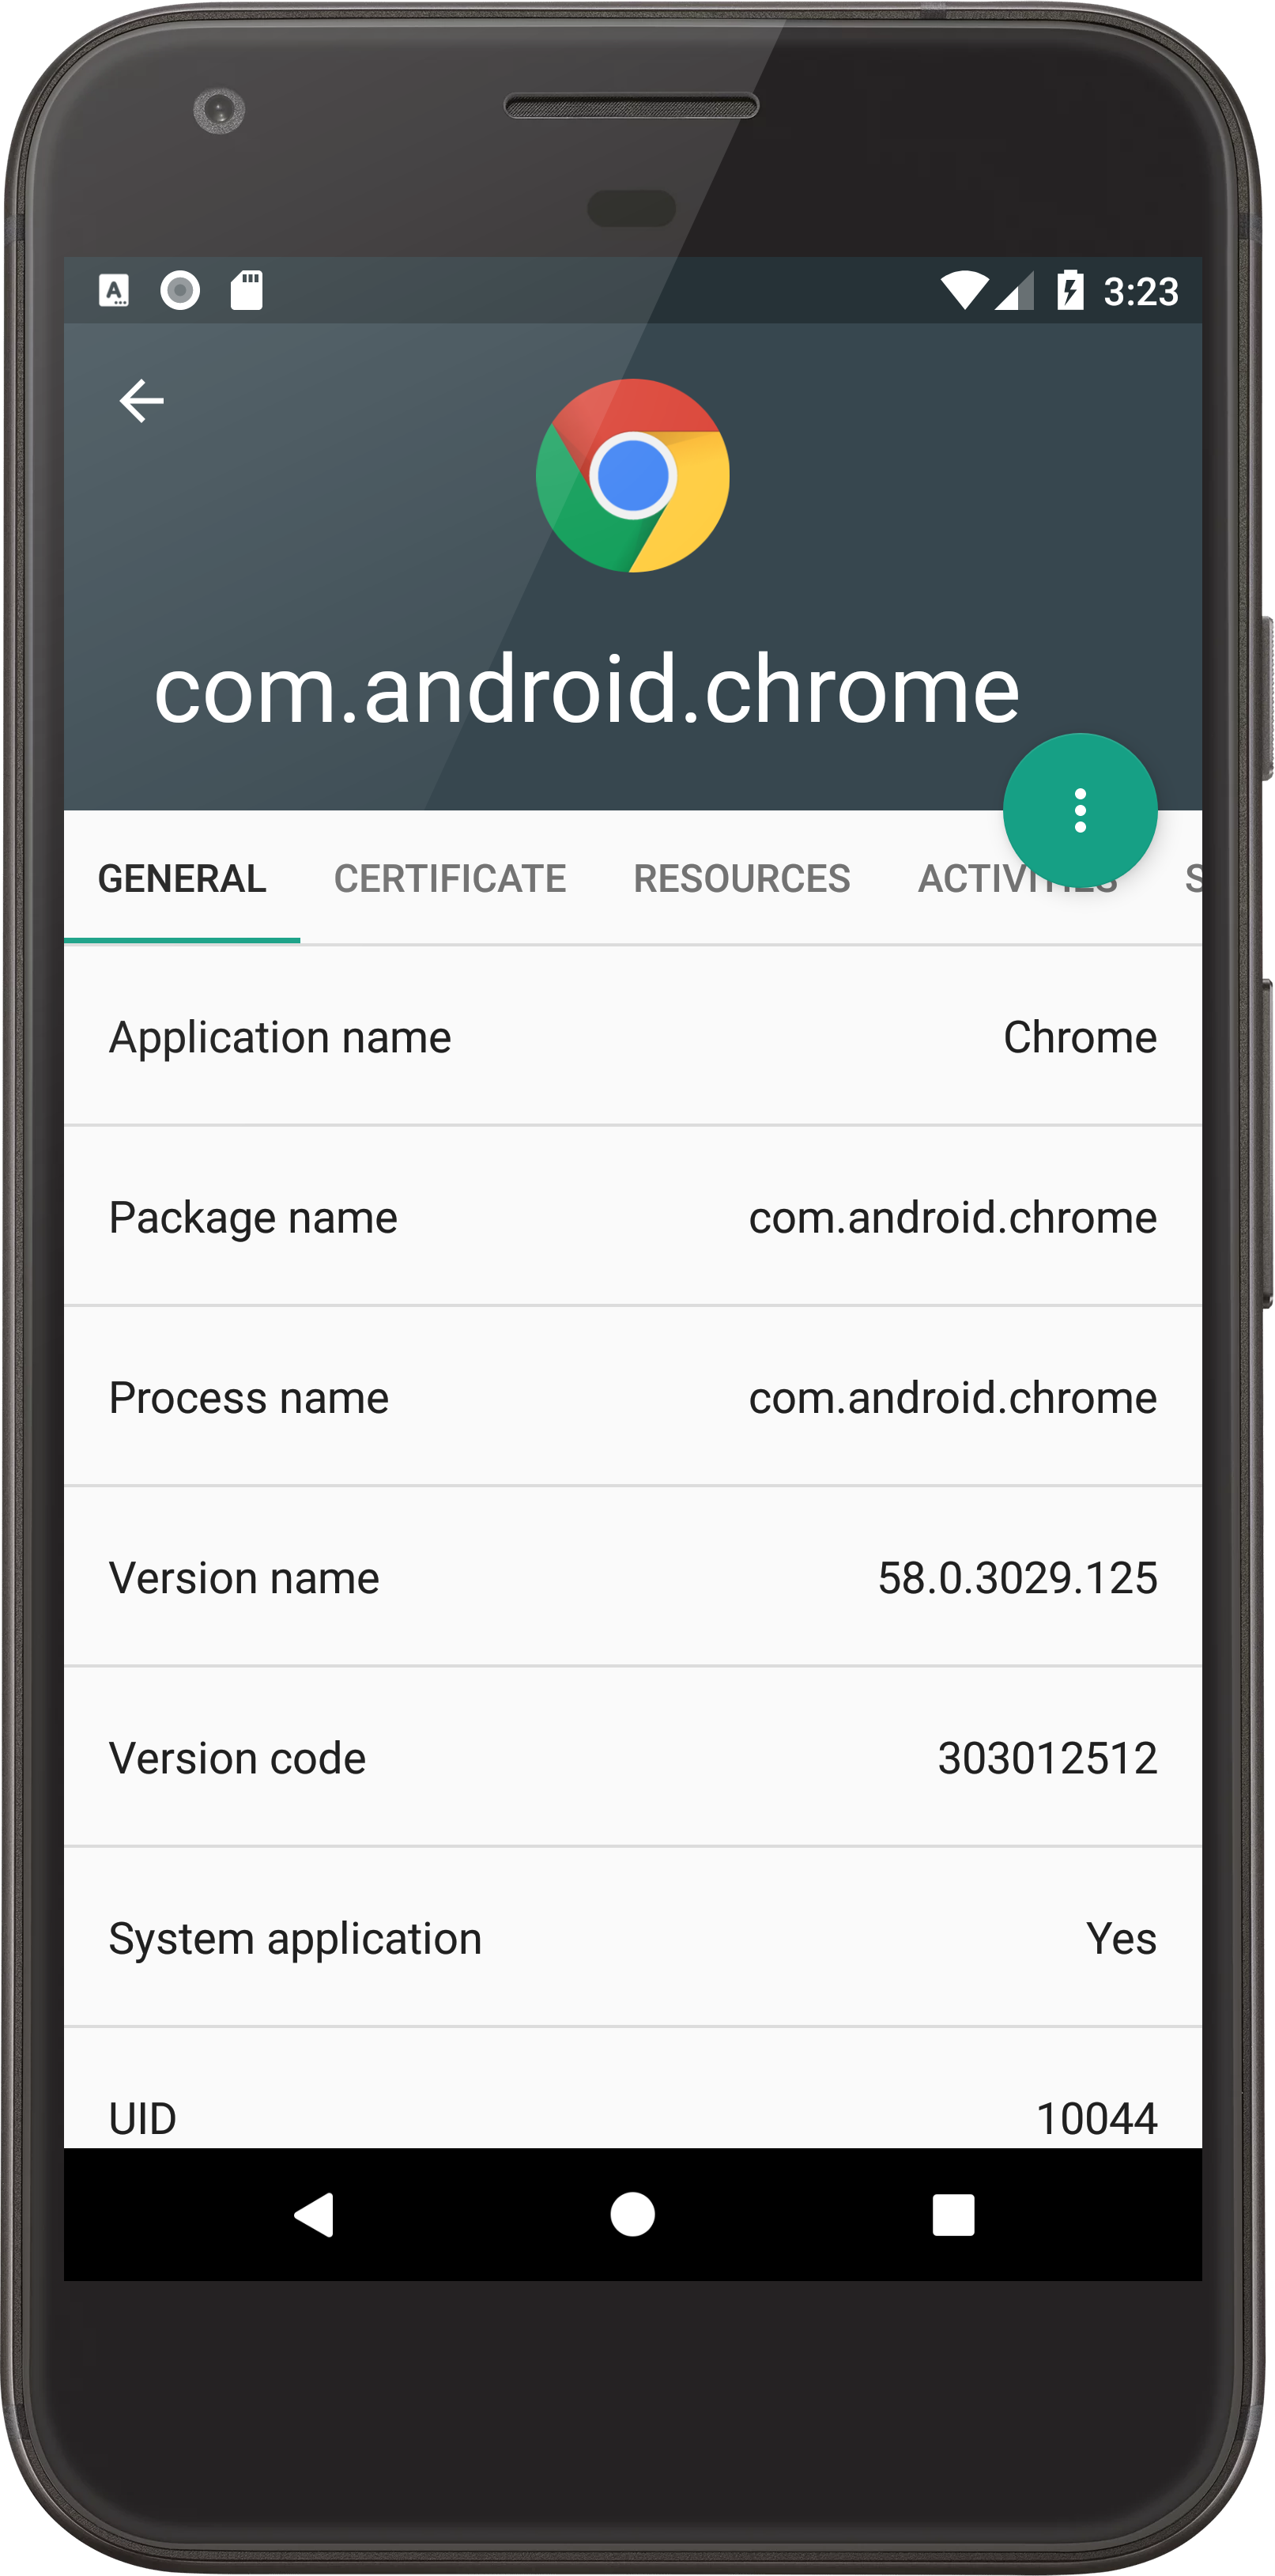
\includegraphics[width=5.2cm]{images/app/detail_device.png}
\centering
\caption{Detaily aplikácie}
\label{fig:app-detail}
\end{minipage}%
\end{figure}

\subsection{Analýza aplikácie pred inštaláciou z lokálneho APK súboru}
Naša aplikácia poskytuje možnosť analýzy pred inštaláciou APK súborov, ktoré sú uložené v lokálnej pamäti zariadenia. Táto funkcionalita je užitočná v prípade stiahnutia aplikácie z webu a jej následnej inštalácie. Po výbere APK súboru pomocou prieskumníka súborov, spustí Android inštaláciu prevzatej aplikácie. V prípade, že má používateľ nainštalovanú našu aplikáciu, nespustí Android inštaláciu automaticky po kliknutí na APK súbor. Namiesto toho zobrazí užívateľovi dialóg, v ktorom si môže vybrať medzi priamou inštaláciou a analýzou v aplikácii \zv{Apk Analyzer}. Naša aplikácia zobrazí detaily APK balíčka a zároveň ponúkne užívateľovi možnosť nainštalovať danú aplikáciu.

\subsection{Štatistické údaje o nainštalovaných aplikáciách}
Obrazovka zobrazujúca štatistické informácie získané analýzou všetkých nainštalovaných aplikácií. Primárnym účelom tejto funkcie je poskytnúť užívateľovi zaujímavý štatistický prehľad o kolekcii jeho aplikácií. 

\noindent Dáta prezentované touto obrazovkou pomocou grafov zahŕňajú:
\begin{itemize}
	\item \bod{Kompatibilné verzie systému Android} -- minimálna a cieľová verzia Android API
	\item \bod{Inštalačné politika aplikácie} -- preferované umiestnenie aplikácie
	\item \bod{Algoritmus podpisu balíčka}
	\item \bod{Pôvod aplikácií} -- rozlíšenie medzi predinštalovanými aplikáciami a aplikáciami z oficiálnych a neoficiálnych zdrojov. 
\end{itemize}
\noindent Po kliknutí na položku grafu je zobrazený zoznam aplikácií, ktoré patria do danej kategórie.

\noindent Nasledujúce dáta sú prezentované pomocou štandardných štatistických ukazovateľov:
\begin{itemize}
	\item Veľkosť aplikácií
	\item Počet komponent aplikácií
	\item Počet súborov
	\item Počet obrazoviek
	\item Počet obrázkov
\end{itemize}
Štatistické dáta o týchto atribútoch zahŕňajú aritmetický priemer, medián, maximálnu a minimálnu hodnotu, rozptyl a smerodajnú odchýlku. 

\subsection{Odosielanie aplikačných metadát na server}
Mobilná aplikácia odosiela metadáta o všetkých nesystémových aplikáciách na server, kde sú tieto dáta použité za účelom detekcie prebalených aplikácií.

Informácie o nainštalovaných aplikáciách sú klasifikované ako citlivé údaje. Tieto dáta nie je možné zbierať bez povolenia od užívateľa. Z tohto dôvodu naša aplikácia počas prvého spustenia požiada užívateľa o súhlas s odosielaním metadát o jeho aplikáciách. Užívateľ má neskôr možnosť zmeniť svoje rozhodnutie v sekcií nastavenia.

V prípade, že užívateľ povolí odosielanie dát a zariadenie je pripojené na internet, aplikácia na pozadí analyzuje všetky nesystémové aplikácie a odosiela dáta na server systému \zv{Apk Analyzer}. Tento proces sa spustí pri každom spustení aplikácie. Dáta sú odosielané v serializovanej podobe vo formáte JSON. Keďže tieto dáta obsahujú hashe všetkých súborov v aplikácii, veľkosť odosielaného súboru môže pri väčších aplikáciách dosiahnuť až 1\,MB. Z dôvodu efektívneho využitia siete sú tieto dáta skomprimované pomocou algoritmu GZIP, ktorý mnohonásobne zmenší veľkosť prenášaných dát.

Server a centrálna databáza neakceptujú viacero záznamov o jednej verzii aplikácie odoslaných z jedného zariadenia. Na identifikáciu zariadenia slúži \zv{Android Id}, ktoré je taktiež súčasťou odosielaných dát. Za účelom zamedzenia odosielania dát, ktoré už boli z daného zariadenia odoslané, využíva naša mobilná aplikácia lokálnu databázu, do ktorej ukladá meno balíčku a verziu všetkých aplikácií, ktoré boli úspešne odoslané na server. Aplikácia je analyzovaná a odosielaná len v prípade, že ju dané zariadenie ešte neodoslalo.

Komunikácia so serverom prebieha prostrednístvom HTTPS a aplikácia sa musí serveru autentizovať.

\subsection{Detekcia prebalenej aplikácie}
Detekcia prebalených aplikácií prebieha na strane serveru a mobilná aplikácia predstavuje len používateľské rozhranie, prostredníctvom ktorého ma užívateľ možnosť požiadať o detekciu svojich aplikácií. Táto funkcia je dostupná z menu obrazovky zobrazujúcej detaily aplikačného balíčku. Výsledky detekcie prezentované užívateľovi obsahujú:
\begin{itemize}
\item Výsledok -- aplikácia je/nie je prebalená, alebo systém nemá dostatok dát na vyhodnotenie
	\item Počet identifikovaných nadmieru podobných aplikácií
	\item Pomer aplikácií od vydavateľa, od ktorého pochádza užívateľov aplikácia a všetkých identifikovaných podobných aplikácií
	\item Pomer aplikácií od vydavateľa, od ktorého pochádza väčšina podobných aplikácií a všetkých identifikovaných podobných aplikácií
\end{itemize}
	
	
